%%%%%%%%%%%%%%%%%%%%%%%%%%%%%%%%%%%%%%%%%%%%%%%%%%%%%%%%%%%%%%%%%%%%%%%%%%%%%%%%
%2345678901234567890123456789012345678901234567890123456789012345678901234567890
%        1         2         3         4         5         6         7         8

\documentclass[letterpaper, 10 pt, conference]{ieeeconf}
\overrideIEEEmargins                                                % Needed to meet printer requirements.
\usepackage[utf8]{inputenc}
\usepackage[T1]{fontenc}
\usepackage{tikz}
\usetikzlibrary{positioning,fit,arrows.meta,backgrounds}
\usepackage{graphicx}
\usepackage{amsmath, amssymb, xcolor, tikz, pgfplots, pgfplotstable}

\newcommand{\todo}[1]{{\color{red}#1}}
\usepackage{listings, xcolor}

\pgfplotsset{compat=1.3}

\colorlet{punct}{red!60!black}
\definecolor{background}{HTML}{EEEEEE}
\definecolor{delim}{RGB}{20,105,176}
\colorlet{numb}{magenta!60!black}

\lstdefinelanguage{json}{
    basicstyle=\normalfont\ttfamily,
    numbers=left,
    numberstyle=\scriptsize,
    stepnumber=1,
    numbersep=8pt,
    showstringspaces=false,
    breaklines=true,
    frame=lines,
    backgroundcolor=\color{background},
    literate=
     *{0}{{{\color{numb}0}}}{1}
      {1}{{{\color{numb}1}}}{1}
      {2}{{{\color{numb}2}}}{1}
      {3}{{{\color{numb}3}}}{1}
      {4}{{{\color{numb}4}}}{1}
      {5}{{{\color{numb}5}}}{1}
      {6}{{{\color{numb}6}}}{1}
      {7}{{{\color{numb}7}}}{1}
      {8}{{{\color{numb}8}}}{1}
      {9}{{{\color{numb}9}}}{1}
      {:}{{{\color{punct}{:}}}}{1}
      {,}{{{\color{punct}{,}}}}{1}
      {\{}{{{\color{delim}{\{}}}}{1}
      {\}}{{{\color{delim}{\}}}}}{1}
      {[}{{{\color{delim}{[}}}}{1}
      {]}{{{\color{delim}{]}}}}{1},
}


\title{\LARGE \bf
A Semi-Automated Software Pipeline for Assembling Collision and Near-Collision Dashcam Footage Datasets
}

\author{
         Ben Upenieks, Chaitanya Varier,\\
         Curtis Duy Kha Phan, Jack David Roberts Williamson,\\
         Nicholas Geofroy, Chengzhong Meng, Vincent-Olivier Roch\\
         \\
         Faculties of Mathematics and Engineering, University of Waterloo\\
         \tt\small ben.upenieks@uwaterloo.ca, cvarier@uwaterloo.ca,
         \\ \tt\small cdkphan@uwaterloo.ca, jdrwilli@uwaterloo.ca,
         \\ \tt\small nicholas.geofroy@uwaterloo.ca, c24meng@uwaterloo.ca, vroch@uwaterloo.ca
}

\begin{document}

\maketitle
\thispagestyle{empty}
\pagestyle{empty}


%%%%%%%%%%%%%%%%%%%%%%%%%%%%%%%%%%%%%%%%%%%%%%%%%%%%%%%%%%%%%%%%%%%%%%%%%%%%%%%%
\begin{abstract}

Over the last decade, emphasis has been made on the need for autonomous vehicles to reduce road collisions and reckless driving. However, research into collision prediction has been slowed by the lack of egocentric collision-oriented datasets. Currently, this type of data is often created through computer generated scenarios \cite{Kim_Lee_Hwang_Suh_2019} due to the dangerous and costly nature of road collisions and data collection equipment. We provide a semi-automated software pipeline to assemble datasets of real vehicle collision events that have been published online to various video repositories. We specifically focus on collecting footage of collisions recorded from front-mounted dashcam video cameras and demonstrate the importance of learning from complex road scenes and conditions globally rather than in one region. Further, we present a small prototype dataset that we have produced using our pipeline which includes egocentric dashcam vehicle footage from all over the world, subject to varying visibilities, varying weather conditions, and varying settings.

\end{abstract}

%%%%%%%%%%%%%%%%%%%%%%%%%%%%%%%%%%%%%%%%%%%%%%%%%%%%%%%%%%%%%%%%%%%%%%%%%%%%%%%%
\section{INTRODUCTION}

In the advent of connected vehicles and autonomous transportation, it has become commonplace to equip vehicles with high-end equipment to facilitate automated collision avoidance systems \cite{Perumal2020LidarBI}.
Using these vehicles to record collision situations has a two-fold cost: both the car and expensive data-gathering equipment are put at risk.
However, we can collect collision data naturally in real driving scenarios through dashcams -- cheap video cameras that can be mounted to a car's dashboard.
Typically used for insurance purposes, dashcams have the added benefit of recording a wide variety of real collisions that are difficult to simulate effectively.
This has led to the creation of many online communities to share videos of these rare situations on websites such as Reddit, YouTube, and Imgur.
We propose that this egocentric dashcam video stream can be leveraged by computer vision systems to act as an affordable and commonplace sensor for automated collision prediction.

In this paper we present a software pipeline to facilitate the collection, processing and annotation of egocentric dashcam videos from various online video repositories to produce datasets that can be used to train deep dashcam collision prediction models.
We aim to generate datasets that are not constrained to any regions or countries but rather provide location-agnostic data that is representative of general, global road and vehicle conditions.
These datasets will also be collision-oriented as the majority of these videos contain collisions for people's viewing.
Current autonomous vehicle data collection techniques typically require astronomically expensive hardware and equipment. Consequently, they are rarely involved in collisions and intentionally not put in high risk environments that may lead to a collision.
Thus, our goal is to capture this data by taking advantage of existing videos of real-world collisions.

The pipeline uses web-scraping techniques to fetch the video data from these websites, along with a set of video metadata, describing the video's contents.
We use this data, in combination with the manually annotated data in order to create a prototype collision dataset of dashcam video samples.
This combination allows us to take advantage of the wide variety of videos available on the Internet while still having reliable data that has been curated manually.
As part of this data, we identify \textit{participants} and \textit{bystanders}, both known as \textit{agents}. Participants are objects that are involved in a collision identified in the metadata, while bystanders are uninvolved objects.

It is worthwhile to note that in collecting samples for our prototype dataset, we do not impose a minimum video resolution threshold. We mitigate this by only collecting samples which contain clearly identifiable agents. This allows us to maximize the amount of data that we can feasibly include in our dataset.

%%%%%%%%%%%%%%%%%%%%%%%%%%%%%%%%%%%%%%%%%%%%%%%%%%%%%%%%%%%%%%%%%%%%%%%%%%%%%%%%
\section{RELATED WORK}

Chan et al. \cite{chan2016anticipating} approach the same problem of collision prediction via egocentric dashcam videos. They propose a novel Dynamic-Spatial-Attention Recurrent Neural Network (DSARNN) that distributes attention to localized and detected vehicles within the video and models temporal dependencies to predict the earliest frame of a potential impending collision. Along with their paper, they have released a dataset of 678 dashcam videos capturing areas in Taiwan. Each video is annotated with vehicle tracking bounding boxes, the vehicles that were involved in the collision and the frame of the collision. We hope to allow researchers to expand on this dataset with location-agnostic data and similar annotations.



%%%%%%%%%%%%%%%%%%%%%%%%%%%%%%%%%%%%%%%%%%%%%%%%%%%%%%%%%%%%%%%%%%%%%%%%%%%%%%%%
\section{AUTODASH 2021}
We aim to provide a dataset that contains a diverse set of egocentric vehicle collision videos with different locations and collision scenarios. In order to source these videos, we built a data pipeline that collects user-submitted videos from YouTube and Imgur. Using our pipeline, we collected and labelled 250 video clips of collision and near-collision scenarios from various locations in Europe, Asia, and North America. We have a variety of scene types such as city streets, highways, and rural areas from these locations. All video clips are annotated with bounding boxes for the vehicles and pedestrians present, as well as frame indices and object IDs for the participants in the collision.

\subsection{Video Collection Pipeline}
In order to facilitate collection of videos, we built a video discovery and annotation pipeline that can be customized for many labelling tasks. Our pipeline is built from several modular components called executors that each process or handle the data corresponding to a single video before piping the resulting data to the next executor using a pipe and filter architecture. The pipeline fetches and stores video metadata as JSON in a NoSQL cloud database and enables concurrent labelling of videos.

We collect a wide range of metadata on each video such as the set of bounding boxes for actors in the video, the object type of all the actors, the start frame of any collision in the video, and the location of the video.

The most basic pipeline configuration starts off with a set of web scrapers that each target and scrape a specific website or video repository based on a user-defined set of key-terms, and a \textit{database source executor} that pulls unlabelled videos from the  database. Videos that are pulled by the scrapers are immediately added to the database in order to ensure only one person is labeling a video at a time.

After a video has been downloaded to the user's machine, it is passed to the \textit{Splitter Executor}, which is used to split an input video into multiple sub-videos. We use the splitter for long-form videos that may contain multiple independent collision events or irrelevant video segments, such as compilation videos or videos with substantial editing and transitions. The \textit{Splitter} outputs a different metadata item for each distinct sub-video extracted from its input video.

After collection and preprocessing, a core component of our pipeline is a GUI tool (Figure \ref{fig:example_gui_tool-png}) that facilitates the manual annotation of the dashcam videos, and quick manual filtering of non-dashcam and irrelevant videos. We provide tools to annotate the video bounding boxes to localize, identify and track agents in the video segment, as well as ways to label the type of each agent and the location of the video. In order to assist with the manual labelling of bounding boxes, we provide ways to linearly interpolate between two user-drawn bounding boxes, so the user does not need to label every frame.

\begin{figure}[htbp]
  \centering
  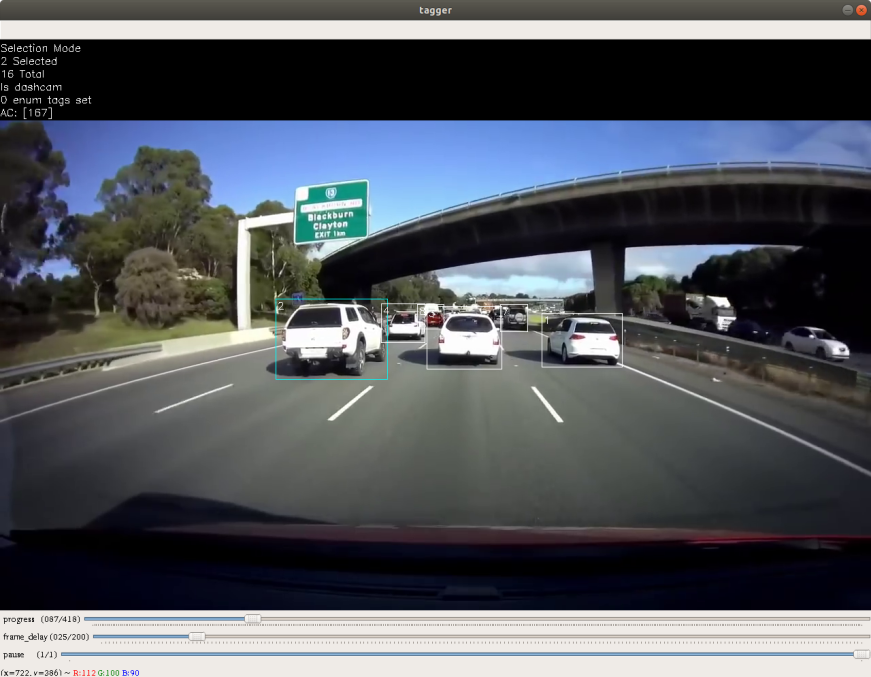
\includegraphics[width=0.46\textwidth]{example_gui_tool.png}
  \caption{GUI tool to facilitate annotation}
  \label{fig:example_gui_tool-png}
\end{figure}

\subsection{Object Detection}
Every video in the dataset contians bounding boxes for all of the actors present in the video. Each actor is given a numerical ID, a list of bounding boxes that contain that actor for every frame they are present, as well as a classificaiton of the actor. There are 9 different classifications with the majority of objects being classified as one of "car", "truck", "van", or "motorcycle"

\subsection{Collision Detection}
Assisting in collision detection algorithms is the main purpose of this dataset, and as such we collect multiple pieces of data about the collision. We label and define a \textit{collision location} as the index of the first frame in the video for which at least one actor makes unintentional contact with another actor or stationary object. A given video may have multiple collision locations, especially in the case of highway scenes, and therefore each metadata contains a list of frame numbers for such events.

In addition to \textit{collision location} we classify every actor $a_i$ in the video with a \textit{has\_collision} flag that specifies if $a_i$ takes part in a collision at any point in the video.

\subsection{Anonymization}
An important facet of automobile data aggregation is in eliminating biases and protecting the identities of depicted individuals. Consequently, our pipeline contains a post-processing stage in which we anonymize personally identifiable information. Specifically, we provide the executor \texttt{FaceBlurrer}, which blurs faces. This executor first uses a MobileNet Single Shot MultiBox Detector \cite{yixuan_h_y_hu_2021_4642275} trained on the WIDERFACE dataset \cite{yang2016wider} to obtain the bounding boxes of all visibly identifiable individuals' faces at each frame of a given video. The executor then applies a blurring mask over each bounding box and writes the modified frame back to the video stream. We have chosen to use a MobileNet SSD for this task because it achieves a good balance between accuracy and performance, while requiring relatively little memory \cite{yixuan_h_y_hu_2021_4642275}.

This software module is encapsulated as a library and can be reused in other projects by importing our \texttt{anonymization} package. The accuracy, amount and type of blurring applied can be tweaked using the exposed API.

%%%%%%%%%%%%%%%%%%%%%%%%%%%%%%%%%%%%%%%%%%%%%%%%%%%%%%%%%%%%%%%%%%%%%%%%%%%%%%%%
\section{EXPERIMENTS}

\subsection{Prototype Dataset}
\label{section-prototype-dataset}
In order to evaluate the importance of acquiring data from multiple geographical locations and under varying driving conditions around the world, we have built a prototype dataset of 223 video clips using our pipeline on which we will test the existing collision anticipation model, DSARNN. This dataset is comprised of 97 positive and 126 negative videos. Most of these videos represent road scenes from North America, Europe and Russia which have noticeably different characteristics than those in Taiwan. To prepare our data we follow the steps outlined by Chan et. al \cite{chan2016anticipating}. Namely, we trim videos such that they are 5 seconds long, sampled at 20 FPS, and the collision occurs at frame 90. This trimming and sampling functionality is provided within the pipeline configuration \texttt{smallcorgi\_exporter.yml}. In our experiments, we train the DSARNN model on features produced by running a pre-trained VGG on each full frame and the cropped objects within the frame \cite{DBLP:journals/corr/SimonyanZ14a}. This is denoted VGG+RNN+F+D-con. in the original publication. We note that this data includes manually annotated bounding boxes, so there will be no error imposed by using automated vehicle detection and localization models.

\pgfplotstableread[col sep=comma]{by-classes.csv}\byclass
\pgfplotstableread[col sep=comma]{by-actors.csv}\byactors
\pgfplotstableread[col sep=comma]{by-agents.csv}\byagents
\pgfplotstableread[col sep=comma]{by-duration.csv}\byduration

We have aggregated some statistics about our database and dataset to help clients understand the pertinent distributions in the data. While these distributions may be representative of online collision footage, they are not necessarily representative of real world collisions. The total number of videos represented by the following tables and histograms is a superset of the number of videos in the final prototype dataset as it includes videos that were ultimately unsuitable for our collision prediction experiments. Thus, we denote this superset as the \textit{pre-processed prototype dataset}.

\begin{table}[!h]
    \caption{Distribution of videos in database by download source}
    \label{vids-by-source}
    \begin{center}
        \begin{tabular}{|c|c|}
            \hline
            Download source & Percentage of videos \\
            youtube.com & \textbf{98.40\%} \\
            imgur.com & 0.85\% \\
            gfycat.com & 0.47\% \\
            streamable.com & 0.28\% \\
            \hline
        \end{tabular}
    \end{center}
\end{table}

\begin{table}[!h]
    \caption{Distribution of videos in pre-processed prototype dataset by geographical region}
    \label{vids-by-region}
    \begin{center}
        \begin{tabular}{|c|c|}
            \hline
            Region & Percentage of videos \\
            North America & 48.13\% \\
            Europe & 24.30\% \\
            Russia & 19.16\% \\
            Asia & 4.67\% \\
            Australia & 3.74\% \\
            \hline
        \end{tabular}
    \end{center}
\end{table}

From Table \ref{vids-by-source}, it is clear that the vast majority of videos that have been processed through our pipeline and cataloged in our database were obtained from YouTube. It can also be seen that the YouTube and Reddit downloaders are capable of scraping various other online repositories such as Imgur, Gfycat and Streamable.

From Table \ref{vids-by-region}, we can see that our pre-processed prototype dataset consists of dashcam footage from a reasonably well-balanced distribution of geographical regions. The dataset mostly consists of samples from North America, Europe and Russia, which complements the dataset presented by Chan. et. al. \cite{chan2016anticipating} well. This also implies a diverse representation in driving conditions due to the various differences in climate and infrastructure amongst these regions.

\begin{figure}[!h]
    \centering
    \begin{tikzpicture}
    \begin{axis}[
    title={Objects by class},
    ylabel={Frequency (\# of objects)},
    ymin=-50,
    ymax=1800,
    xtick=data,
    xticklabels from table={\byclass}{X},
    xticklabel style={rotate=50,anchor=east,yshift=-2mm}
    ]
    \addplot[fill, ybar] table [x expr=\coordindex, y={Y}] \byclass;
    \end{axis}
    \end{tikzpicture}
    \caption{Distribution of videos in pre-processed prototype dataset by object class}
    \label{fig:obj-by-class}
\end{figure}

\begin{figure}[!h]
    \centering
    \begin{tikzpicture}
    \begin{axis}[
    title={Videos by participant},
    xlabel={Number of participants},
    ylabel={Frequency (\# of videos)},
    ymin=-5,
    ymax=175,
    xtick=data,
    xticklabels from table={\byactors}{X},
    xticklabel style = {rotate=45,anchor=east,yshift=-2mm}
    ]
    \addplot[fill, ybar] table [x expr=\coordindex, y={Y}] \byactors;
    \end{axis}
    \end{tikzpicture}
    \caption{Distribution of videos in pre-processed prototype dataset by number of participants}
    \label{fig:vids-by-participant}
\end{figure}

From Figure \ref{fig:obj-by-class}, we see that there are several types of objects which have been identified as agents in our pre-processed prototype dataset. Among these, the most common are motorized vehicles and pedestrians as one would intuitively expect. A number of stationary, inanimate objects such as industrial machinery were worth noting as they were involved in collisions. These have been aggregated into the "other" category.

From Figure \ref{fig:vids-by-participant}, it can be seen that there is a wide range in the distribution of the number of participants in each sample of our dataset. We also observe that it is more common for no collisions to occur than any particular non-zero number of participants to be present in a sample.

From Figure \ref{fig:vids-by-agents}, we observe that it is most common for samples to contain either exactly 2 agents or no agents at all. This is implied by the fact that videos with only 1 agent cannot contain a collision. These are less likely to be interesting and in turn, scraped by our pipeline.

\begin{figure}[!h]
    \centering
    \begin{tikzpicture}
    \begin{axis}[
    title={Videos by agents},
    xlabel={Number of agents},
    ylabel={Frequency (\# of videos)},
    ymin=-10,
    ymax=270,
    xtick=data,
    xticklabels from table={\byagents}{X}
    ]
    \addplot[fill, ybar] table [x expr=\coordindex, y={Y}] \byagents;
    \end{axis}
    \end{tikzpicture}
    \caption{Distribution of videos in pre-processed prototype dataset by number of agents}
    \label{fig:vids-by-agents}
\end{figure}

From Figure \ref{fig:vids-by-duration}, we can clearly see that there is a roughly standard normal distribution in the number of videos by duration, with a mean, median and mode at around 352 frames. This suggests that the pipeline favors videos which tend to be shorter on average. At an average video framerate of 30 FPS, this equates to a mean sample duration of just over 11 seconds. In section \ref{section-prototype-dataset}, it was mentioned that the samples were cropped to 5 seconds in the final prototype dataset. Therefore, this is a favorable characteristic as it helps reduce the amount of necessary processing.

\begin{figure}[!h]
    \centering
    \begin{tikzpicture}
    \begin{axis}[
    title={Videos by duration},
    xlabel={Duration (in frames)},
    ylabel={Frequency (\# of videos)},
    xtick=data,
    ymin=-5,
    ymax=130,
    xticklabels from table={\byduration}{X},
    xticklabel style = {rotate=45,anchor=east,yshift=-2mm}
    ]
    \addplot[fill, ybar] table [x expr=\coordindex, y={Y}] \byduration;
    \end{axis}
    \end{tikzpicture}
    \caption{Distribution of videos in pre-processed prototype dataset by duration}
    \label{fig:vids-by-duration}
\end{figure}

Figures \ref{fig:vids-by-collision} and \ref{fig:vids-by-camera} outline key characteristics about our database at large. Figure \ref{fig:vids-by-collision} shows that from the video repositories we targeted, we were able to obtain a relatively well-balanced distribution of collision types in our data. Here, the distinction between \textit{Simple Collision} and \textit{Multi Collision} is that the former involves exactly 2 participants and the latter involves more than 2 participants. Figure \ref{fig:vids-by-camera} shows that the majority of the videos the pipeline scraped were indeed dashcam videos. This suggests that the pipeline is quite effective in identifying suitable candidates for a  dataset consisting solely of dashcam collision footage.

\begin{figure}[!h]
    \centering
    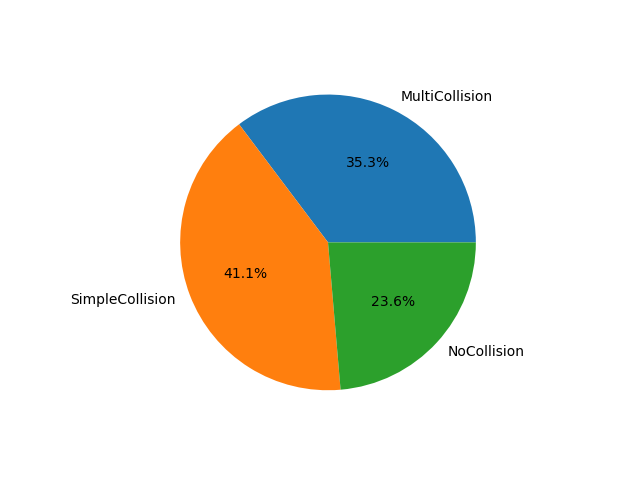
\includegraphics[width=0.46\textwidth,trim={0 1cm 0 0},clip]{by-collision.png}
    \caption{Distribution of videos in database by collision type}
    \label{fig:vids-by-collision}
\end{figure}

\begin{figure}[!h]
    \centering
    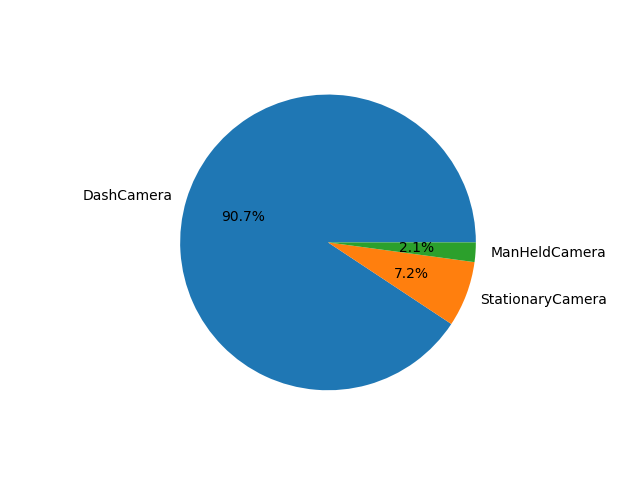
\includegraphics[width=0.46\textwidth,trim={0 1cm 0 1cm},clip]{by-camera.png}
    \caption{Distribution of videos in database by camera type}
    \label{fig:vids-by-camera}
\end{figure}

\subsection{Collision Prediction Model Training and Analysis}
\label{section-collision-prediction}
In our first experiment, we merge our prototype dataset with the dataset provided by Chan et. al. We augment their training set with 77 positives and 106 negatives, and their testing set with 20 positives and 20 negatives. We use the same training procedure as Chan et. al. Namely, we train for 40 epochs with a learning rate of $10^{-4}$ and a batch size of 10. Although our data contribution here is relatively small, we observe a mean time-to-collision of \textbf{2.198s} at \textbf{80\%} recall which is very similar to the existing results from Chan et. al. However, we observe an average precision of 66.22\% which is appreciably lower than the 73.53\% average precision reported by Chan et. al. \cite{chan2016anticipating}

In our second experiment, we use the provided pre-trained DSARNN model and test the performance on our entire dataset of 223 videos. We see very poor prediction performance at an average precision of 34.29\%, and in Figure \ref{fig:pr_curve} we observe poor precision at all recall values.

\begin{figure}[!htbp]
        \centering
        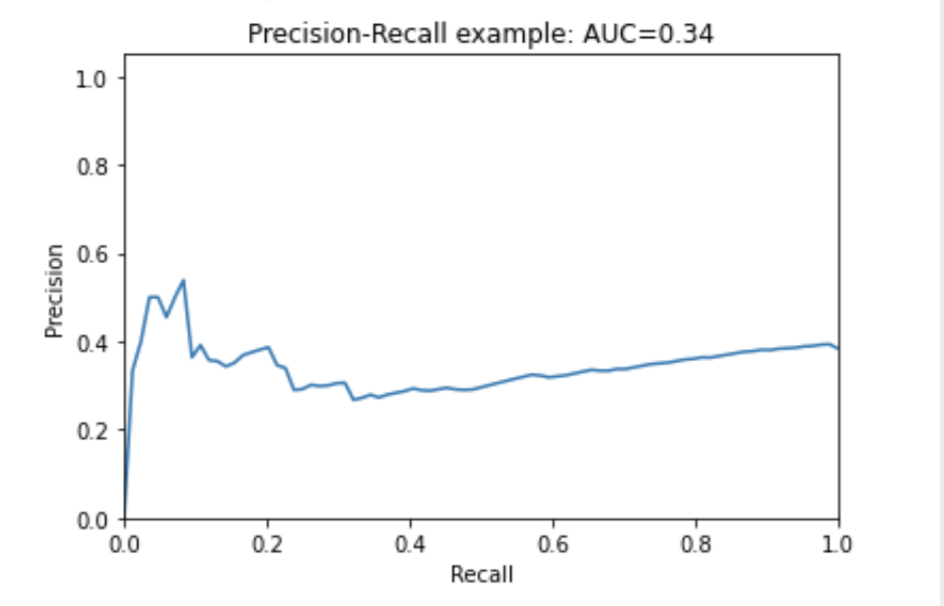
\includegraphics[width=0.5\textwidth]{prcurve.png}
        \caption{Pre-trained DSARNN Precision-Recall curve on prototype dataset}
        \label{fig:pr_curve}
\end{figure}

These experiments support the notion that in order for a collision prediction model to be generally effective in practice, it must be trained on collisions and complex roads scenes from varying regions and road conditions around the world.

%%%%%%%%%%%%%%%%%%%%%%%%%%%%%%%%%%%%%%%%%%%%%%%%%%%%%%%%%%%%%%%%%%%%%%%%%%%%%%%%
%\section{CONCLUSION}
% REMOVED BECAUSE WE DON'T HAVE ANY RESULTS
%\todo{Write the conclusion}
%A conclusion section is not required. Although a conclusion may review the main points of the paper, do not replicate the abstract as the conclusion. A conclusion might elaborate on the importance of the work or suggest applications and extensions.

%%%%%%%%%%%%%%%%%%%%%%%%%%%%%%%%%%%%%%%%%%%%%%%%%%%%%%%%%%%%%%%%%%%%%%%%%%%%%%%%
\section{FUTURE WORK}

There are many ways in which we could improve our system, namely the following:
\begin{enumerate}
\item \textbf{Labelling precision improvements:} The current video labelling process in the pipeline involves manual bounding box drawing with linear interpolation between input frames. This is prone to inserting mistaken bounding boxes that do not exactly match up with the location of an object on certain frames. Automated labelling and custom interpolation would speed up the process of labelling and minimize the cases of misplaced bounding boxes. Labelling would be much faster if we had a semi-automated process of detecting objects and tracking them over frames. There are models for object detection that behave reasonably well for our purposes, but they would still need to be augmented by a review process. We could easily solve the problem of object tracking by implementing simple heuristic algorithms. Being able to modify the method of interpolation between frames beyond the default linear interpolation would allow for more bounding box precision between large input frame windows. Moreover, if we store the interpolation type in the metadata, we would likely gain a significant improvement in performance and memory usage by not storing all the interpolated frames rather than just the ones the user has entered. While linear interpolation works well for entering one frame for every 10 frames in a video clip, supporting additional types of interpolation would facilitate quicker data entry and enable the possibility of supporting affine transformations on more complex bounds.

\item \textbf{Complete Location-Varied Dataset:} Our next step is to expand our existing dataset of automobile collisions to include samples from additional regions across the globe. We would then use this to form a training and testing set for our next experiment. Finally, we would compare the results of this experiment with location-varied data to the results from the dataset collected in Taiwan by Chan et. al.

\end{enumerate}

\addtolength{\textheight}{-12cm}

%%%%%%%%%%%%%%%%%%%%%%%%%%%%%%%%%%%%%%%%%%%%%%%%%%%%%%%%%%%%%%%%%%%%%%%%%%%%%%%%

\nocite{*}
\bibliographystyle{IEEEtran}
\bibliography{IEEEabrv,sources}

\end{document}


